\documentclass[journal]{IEEEtran}

\usepackage[T1]{fontenc}
\usepackage{amsmath,amssymb}
\usepackage{graphicx}
\usepackage{booktabs}
\usepackage{multirow}
\usepackage{siunitx}
\usepackage{tikz}
\usepackage{pgfplots}
\pgfplotsset{compat=1.17}
\usetikzlibrary{shapes.geometric,arrows.meta,positioning,fit}
\usepackage{algorithm}
\usepackage{algpseudocode}
\usepackage{url}
\usepackage{xcolor}

\sisetup{detect-weight=true, detect-family=true}

\begin{document}

\title{From Feasibility to a Measured Timetable: A Taasika-to-UniTime Pipeline at a Computer Engineering Department}

\author{Mihir~Shah, Riya~Kulkarni, Ved~Mundhada, and Akshay~Sathaye\\
\textit{Department of Computer Engineering, COEP Technological University, Pune, India}\\
\textit{Guide: Abhijit A.\ M.}}

\markboth{Preprint, COEP Technological University}{Shah \MakeLowercase{\textit{et al.}}: Taasika-to-UniTime Pipeline}

\maketitle

\begin{abstract}
University course timetabling is an NP-hard assignment problem in which classes, instructors, student cohorts, and rooms must be placed in a weekly grid subject to hard and soft constraints. A preceding feasibility study had shown that UniTime, an open-source constraint-driven scheduling system built on the CPSolver library, can express every scheduling rule in force at a Computer Engineering department without relaxation, but it stopped short of producing a timetable from institutional data. This paper reports the phase that closed that gap. A reproducible pipeline converts a snapshot of the department's existing scheduling database into the sixteen ordered XML documents that UniTime's Data Exchange interface requires, covering one academic session, 56 course offerings comprising 291 classes, 115 instructors, 42 rooms, and a simulated body of 1{,}130 students carrying 9{,}148 section enrolments. An independent evaluator, cross-validated against a second, Java-based implementation to exact agreement, re-derives every reported quantity from the input files rather than from the solver's own counters, because a solver cannot be audited with its own figures. Using this evaluator we show that several earlier runs reporting zero student conflicts were each an artefact of silent re-sectioning, an already-solved instance, or an empty student population. Once enrolments were pinned, the final solution placed 290 of 291 classes with no instructor or room double-booking, a hard feasibility score of 98.85 out of 100, and 40 of 1{,}130 students carrying a genuine timetable clash, all first-year students in one laboratory--lecture pairing. A reinforcement-learning layer that selects among eight CPSolver neighbourhood operators was also implemented and instrumented; its pre-registered control experiment showed that simply raising the solver's student-conflict weight already clears the improvement threshold the learned policy had been set to beat, so no claim is made that learning outperforms a correctly tuned baseline on this instance.
\end{abstract}

\begin{IEEEkeywords}
course timetabling, constraint programming, UniTime, CPSolver, iterative forward search, student conflicts, reinforcement learning.
\end{IEEEkeywords}

\section{Introduction and Problem Statement}
\label{sec:intro}

Course timetabling at a university requires assigning a large number of classes---each with its own room, instructor, and duration requirements---to slots in a weekly grid, subject to a wide variety of hard and soft constraints. The problem is NP-hard: no polynomial-time exact algorithm is known, and practical systems rely on heuristic or metaheuristic search~\cite{schaerf1999survey}.

The Department of Computer Engineering at COEP Technological University presents a demanding instance of this problem. It runs four undergraduate years and a postgraduate programme, each split into lecture divisions and further into laboratory batches, overlaid with departmental electives, minor-degree courses taught by other departments, open electives, and reserved first-year blocks. Laboratory sections of a course run in parallel while its lectures run jointly, so the natural scheduling unit is neither the course nor the student but the section, and the relationships between sections are what make a timetable usable or useless.

A preceding feasibility study evaluated UniTime, an open-source, web-based academic scheduling system built on the CPSolver constraint library, as a candidate platform. It deployed the system locally, entered representative test data, and mapped the institution's scheduling rules onto UniTime's constraint model, concluding that every identified rule was expressible without relaxation or external post-processing. That conclusion was a statement about the platform, not about a timetable: no institutional data had been loaded, no solution had been produced from real course structure, and no measurement of solution quality existed. The data pipeline, the student records, and the evaluation framework were all still in the future tense.

Closing that gap matters for reasons beyond this one department. A constraint model that can \emph{express} every institutional rule says nothing about whether a real snapshot of a real scheduling database can be turned into solver input without manual re-entry, whether the resulting schedule is actually good by any measure the institution cares about, or whether that measure can be trusted at all. All three questions turn out to have non-obvious answers here, and the third is the one this paper spends the most space on, because a scheduling system that quietly reports a better number than the timetable deserves is arguably worse than one that reports an honestly mediocre one: the first invites a decision-maker to stop looking for a problem that is still there.

The present phase, carried out under the project name \emph{taasika-v3}, closes that gap. Its contributions are:
\begin{enumerate}
\item a reproducible pipeline that reads a snapshot of the department's existing \emph{Taasika} scheduling database and emits the sixteen ordered XML documents that UniTime's Data Exchange interface consumes;
\item institution-specific rules---minor-degree and open-elective time blocks, division and batch structure, and dynamic lunch breaks for students and instructors---encoded as generated preference data rather than entered by hand;
\item an independent evaluation framework that scores any exported timetable against the same input data, because a solver's own quality report cannot be used to audit the solver;
\item an honest account of solution quality, in which several configurations that reported zero student conflicts are each shown to be an artefact rather than an improvement, and a final, pinned-enrolment solution is reported in its place; and
\item a reinforcement-learning layer that selects among stock CPSolver neighbourhood operators, whose pre-registered control experiment answers its own research question in the negative.
\end{enumerate}

\subsection{Related work}
Automated timetabling has a long history as a constraint-satisfaction and optimisation problem, and surveys of the field consistently identify constraint programming and local search as the dominant methodologies for university course timetabling, precisely because they can mix mandatory and preferential requirements within a single model~\cite{schaerf1999survey}. UniTime and its embedded solver, CPSolver~\cite{cpsolver}, are one mature instance of that approach: CPSolver combines Iterative Forward Search with Conflict-based Statistics~\cite{muller2004constraint} and has performed competitively in international timetabling competitions~\cite{muller2009itc,muller2025itc}, and the minimal-perturbation formulation developed alongside it specifically addresses the practical requirement that a re-solved timetable should disturb as few existing placements as possible~\cite{muller2007minimal}. The mapping from an institution's offerings, subparts and sections onto that model is set out by Murray, M\"uller and Rudov\'a~\cite{murray2007modeling}; later accounts describe the same system in daily use~\cite{rudova2011complex}, including elective courses and multiple sections~\cite{muller2016curriculum}. Soft requirements are carried as weighted criteria rather than as further hard constraints~\cite{rudova2003soft}. What is less documented in the published literature is the \emph{operational} path from an institution's own legacy scheduling database into such a system, and, more importantly, how easily a scheduler's reported conflict count can be made to look better than the timetable actually is once students are allowed to move between sections. That operational gap, rather than a gap in the constraint model itself, is the subject of this paper: the preceding feasibility phase of this project already established that the model is adequate, and what remained open was whether a working pipeline could be built on top of it and whether its output could be measured honestly.

\subsection{Scheduling model}
In the CPSolver course-timetabling model the decision variable is a class---a single lecture, laboratory, or tutorial section---and its value is a placement: a starting time together with the room or rooms in which the class meets. Students are not decision variables. A student's timetable is a consequence of the placements chosen for the classes that student is enrolled in, and the cost of two classes overlapping for a shared cohort is priced through a joint-enrolment constraint between those two classes. The solver can therefore only improve a student's timetable by moving a class or, if permitted, by moving the student into a different section---and it is exactly this second mechanism that later sections show to be a source of illusory improvement. Student sectioning is otherwise a problem in its own right~\cite{muller2010sectioning}, not a side effect of the timetable.

Hard constraints must hold in any acceptable timetable: no room or instructor hosts two overlapping classes; a class is placed only in a room whose capacity and type suit it; every class respects its declared meeting pattern and the term's date pattern; and weekends are excluded. Soft constraints express quality rather than legality: preferred rooms and times, balanced instructor load, limited back-to-back teaching, a protected lunch window, and---the criterion this paper treats as primary---the number of students whose personal timetable contains an overlap.

\subsection{The measurement problem}
\label{sec:measurement-problem}
The central difficulty of this phase was not producing a feasible timetable; coverage, room, and instructor feasibility were reached early. The difficulty was that student-conflict counts could not be trusted, because three mechanisms independently drive the reported figure toward zero without improving any student's timetable: \emph{re-sectioning}, in which UniTime moves students between parallel laboratory batches until overlaps disappear while the placements themselves stay unchanged; an \emph{empty student population}, under a demand setting that loads zero students and reports a conflict count of zero over an empty denominator; and a \emph{denominator mismatch}, in which a conflict rate computed over the students who carry enrolments in a solver export is not comparable to one computed over every student in the source data. Sections~\ref{sec:evaluator} and~\ref{sec:results} treat the problem as two objectives rather than one: produce a feasible timetable, and establish a measurement of student conflicts that none of these three mechanisms can satisfy.

\subsection{Solver mechanics}
The embedded solver, CPSolver, is a local-search framework with constraint-programming primitives, built on Iterative Forward Search (IFS)~\cite{muller2004constraint}. IFS differs from classical local search in that it operates over feasible yet potentially incomplete solutions: some classes may remain unassigned, but every hard constraint holds for the classes that are assigned, so an intermediate solution is always interpretable by a human scheduler. From an initial timetable, each iteration selects a class and a placement, removes the assignments that hard-conflict with it, installs the new one, and keeps the best timetable seen so far. Fig.~\ref{fig:ifs} shows the loop as it actually runs in this project's configuration, including the distinction between proposing a move and committing it; the reinforcement-learning layer of Section~\ref{sec:rl} replaces only the \emph{Propose move} step. That step draws one assignment from the neighbourhood of the current one, the mechanism described in M\"uller's thesis~\cite{muller2005thesis}. CPSolver exposes the choice of neighbourhood through its \texttt{NeighbourSelection} extension point. The time changes, room changes and swaps used by the competition solver are described in~\cite{muller2009itc}, and later changes to that set in~\cite{muller2016evolution}. A proposed move is accepted or rejected by a great-deluge rule~\cite{dueck1993deluge}. IFS is augmented with Conflict-based Statistics (CBS)~\cite{muller2004constraint}, which record how often each assignment has historically caused a hard conflict with another and penalise candidate placements accordingly during value selection, steering the search away from historically problematic regions. In the configuration used throughout, \texttt{Basic.DisobeyHard} is \texttt{false}, so every mechanism described later inherits the guarantee that hard constraints are never violated by a persisting assignment.

\begin{figure}[t]
\centering
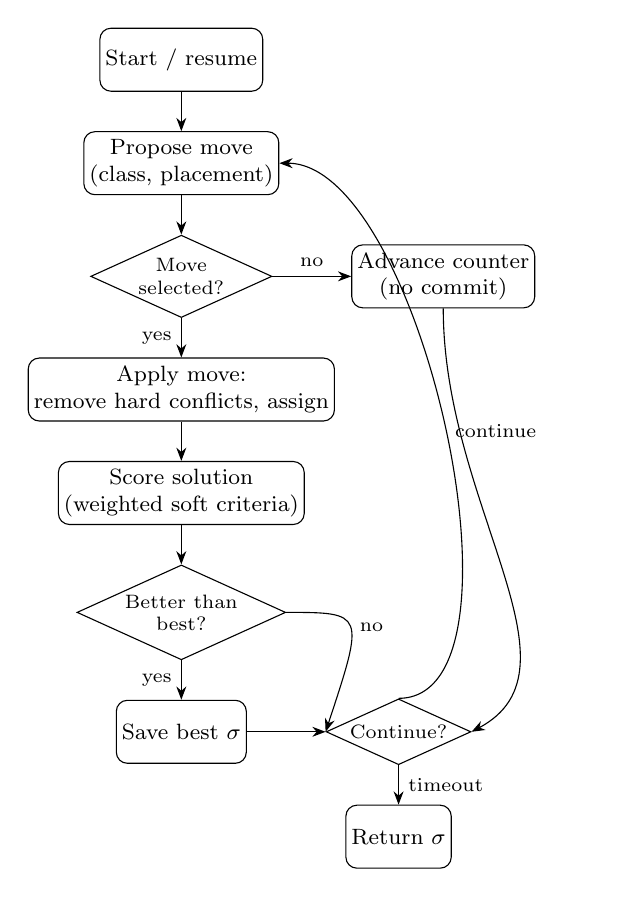
\begin{tikzpicture}[
    node distance=5mm and 6mm,
    box/.style={draw, rounded corners, align=center, minimum height=8mm, font=\footnotesize, inner sep=2pt},
    dec/.style={draw, diamond, aspect=2.2, align=center, font=\scriptsize, inner sep=1pt},
    >=Stealth
]
\node[box] (start) {Start / resume};
\node[box, below=of start] (propose) {Propose move\\(class, placement)};
\node[dec, below=of propose] (hasmove) {Move\\selected?};
\node[box, below=of hasmove] (apply) {Apply move:\\remove hard conflicts, assign};
\node[box, below=of apply] (score) {Score solution\\(weighted soft criteria)};
\node[dec, below=of score] (better) {Better than\\best?};
\node[box, below=of better] (save) {Save best $\sigma$};
\node[box, right=10mm of hasmove] (advance) {Advance counter\\(no commit)};
\node[dec, right=10mm of save] (cont) {Continue?};
\node[box, below=of cont] (ret) {Return $\sigma$};

\draw[->] (start) -- (propose);
\draw[->] (propose) -- (hasmove);
\draw[->] (hasmove) -- node[left, font=\scriptsize]{yes} (apply);
\draw[->] (hasmove) -- node[above, font=\scriptsize]{no} (advance);
\draw[->] (apply) -- (score);
\draw[->] (score) -- (better);
\draw[->] (better) -- node[left, font=\scriptsize]{yes} (save);
\draw[->] (save) -- (cont);
\draw[->] (better.east) .. controls +(10mm,0) .. node[right, font=\scriptsize]{no} (cont.west);
\draw[->] (advance.south) .. controls +(0,-25mm) and +(15mm,8mm) .. (cont.east);
\draw[->] (cont) -- node[right, font=\scriptsize]{timeout} (ret);
\draw[->] (cont.north) .. controls +(18mm,0) and +(18mm,0) .. node[right, font=\scriptsize]{continue} (propose.east);
\end{tikzpicture}
\caption{The CPSolver Iterative Forward Search loop as configured in this project. The incumbent $\sigma$ is updated only when the comparator judges the new solution better. The reinforcement-learning layer of Section~\ref{sec:rl} substitutes only the \emph{Propose move} step.}
\label{fig:ifs}
\end{figure}

Within UniTime a course is modelled hierarchically: an instructional offering carries one or more configurations, each configuration contains scheduling subparts (for example a lecture subpart and a laboratory subpart), and each subpart contains the classes actually placed in the timetable. This hierarchy is what lets a course with joint lectures and parallel laboratory batches be represented as a single offering, and it is why the institution's division-and-batch structure maps onto UniTime without distortion.

\section{Data and Institution-Specific Constraints}
\label{sec:data}

\subsection{Source system and pipeline}
\emph{Taasika} is the scheduling database already in use at the institution. A SQL dump of it stores the data as a series of numbered snapshots, each a complete picture of the departmental schedule at a point in time. A deliberate design decision was to parse the dump textually rather than restore it into a database server: the loader reads the dump and exposes each table as a list of records filtered to a chosen snapshot, so the pipeline has no database dependency and treats the dump as immutable input.

Fig.~\ref{fig:pipeline} shows the complete path from the SQL dump to a scored timetable. Eight generator modules run in dependency order, covering the session, curriculum structure, rooms, instructors, course offerings, scheduling preferences, and a simulated student body; three validators check the result; and an archive step produces the ZIP file that UniTime's Data Exchange page accepts. The sixteen documents must be imported in a fixed order because each later file references entities created by an earlier one---most importantly, the time-pattern and date-pattern preferences must precede the student records, or UniTime treats classes as "arrange hours" and never loads them into the solver at all.

\begin{figure}[t]
\centering
\resizebox{\linewidth}{!}{%
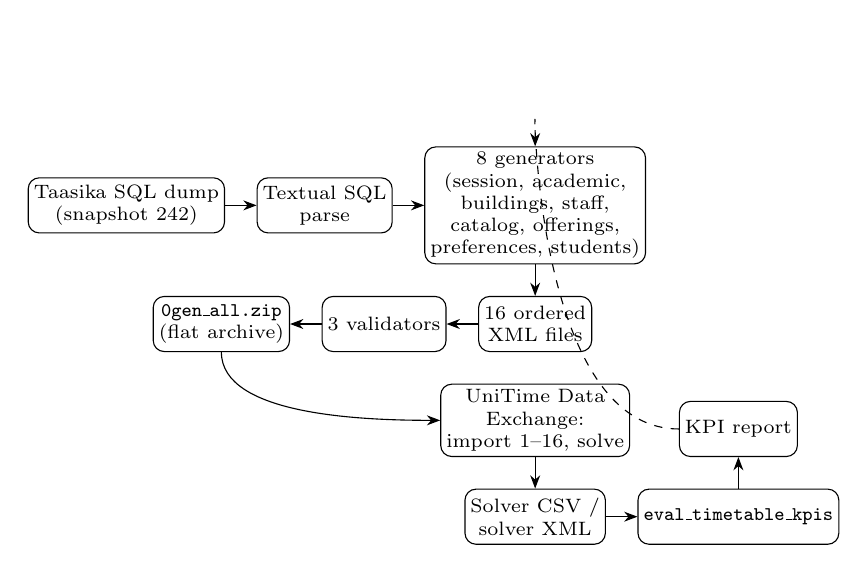
\begin{tikzpicture}[
    node distance=4mm and 4mm,
    box/.style={draw, rounded corners, align=center, font=\scriptsize, inner sep=2pt, minimum height=7mm},
    >=Stealth
]
\node[box] (sql) {Taasika SQL dump\\(snapshot 242)};
\node[box, right=of sql] (loader) {Textual SQL\\parse};
\node[box, right=of loader] (gen) {8 generators\\(session, academic,\\buildings, staff,\\catalog, offerings,\\preferences, students)};
\node[box, below=of gen] (xml) {16 ordered\\XML files};
\node[box, left=of xml] (val) {3 validators};
\node[box, left=of val] (zip) {\texttt{0gen\_all.zip}\\(flat archive)};
\node[box, below=of xml] (import) {UniTime Data\\Exchange:\\import 1--16, solve};
\node[box, below=of import] (export) {Solver CSV /\\solver XML};
\node[box, right=of export] (eval) {\texttt{eval\_timetable\_kpis}};
\node[box, above=of eval] (report) {KPI report};

\draw[->] (sql) -- (loader);
\draw[->] (loader) -- (gen);
\draw[->] (gen) -- (xml);
\draw[->] (xml) -- (val);
\draw[->] (val) -- (zip);
\draw[->] (zip.south) .. controls +(0,-8mm) and +(-10mm,0) .. (import.west);
\draw[->] (import) -- (export);
\draw[->] (export) -- (eval);
\draw[->] (eval) -- (report);
\draw[->, dashed] (report.west) .. controls +(-20mm,0) and +(0,15mm) .. (gen.north);
\end{tikzpicture}}
\caption{The taasika-v3 pipeline. Data flows from the SQL snapshot to a scored timetable; the dashed return path is the refinement loop of Section~\ref{sec:evaluator}.}
\label{fig:pipeline}
\end{figure}

\subsection{Dataset}
The working dataset, \texttt{unitime-out/0gen\_all}, carries the term attribute \texttt{Spr12} and year 2026 throughout, giving the Data Exchange term identifier \texttt{Spr122026}. It was generated from Taasika snapshot 242 (named \texttt{published-v4-26jan26}), identified by cross-checking entity counts against the source database rather than trusted from the file metadata: four of the generated documents carry a hard-coded attribute naming snapshot 240, a stale string left over from an earlier generator version and not updated when a different snapshot is selected. Snapshot 242 is correct and is the snapshot used for every figure in this paper.

Table~\ref{tab:inventory} gives the dataset inventory, recomputed directly from the generated files.

\begin{table}[t]
\centering
\caption{Inventory of \texttt{unitime-out/0gen\_all} (term Spr122026).}
\label{tab:inventory}
\footnotesize
\begin{tabular}{@{}lll@{}}
\toprule
File & Contents \\
\midrule
1sessionSetup & session, departments, subject areas, patterns \\
2academicArea & 2 areas (B.Tech, M.Tech) \\
3academicClassification & 5 year codes (FY, SY, TY, BT, MT) \\
4Major / 5Minor & 15 majors; minors modelled as majors \\
6studentGroup & 242 groups (43 classes + 199 batches) \\
7buildingRoomImport & 6 buildings, 42 rooms \\
8roomSharing & 45 sharing blocks; weekends unavailable \\
9travelTimes & 7 inter-building travel entries \\
10staff & 115 instructors \\
11courseCatalog & 158 courses \\
12courseOffering & 56 offerings, 84 subparts, 291 classes \\
13preferences & 362 preference blocks \\
14studentInfo & 1{,}130 students, 5{,}767 group refs. \\
15studentRequest & requests for 1{,}130 students \\
16studentenrollments & 9{,}148 section enrolments \\
\bottomrule
\end{tabular}
\end{table}

Table~\ref{tab:population} gives the simulated student population. Institutional MIS data was not available, so the student body is simulated from headcounts confirmed with the department: the simulation allocates students to lecture divisions, then to laboratory batches, then issues a course request for every compulsory subject and one per elective group, and finally enrols each student in a concrete lecture and laboratory section. No real student data appears anywhere in the dataset; synthetic identifiers are used throughout.

\begin{table}[t]
\centering
\caption{Simulated student population of the current dataset.}
\label{tab:population}
\footnotesize
\begin{tabular}{@{}lrrl@{}}
\toprule
Year & CSE & AI\&ML & Total / structure \\
\midrule
First year (FY) & 300 & 100 & 400, single cohort \\
Second year (SY) & 200 & 0 & 200, two lecture divisions \\
Third year (TY) & 200 & 0 & 200, two divisions \\
Final year (BT) & 200 & 0 & 200, two divisions \\
M.Tech (MT) & \multicolumn{2}{c}{130} & specialisation streams \\
\midrule
Total & \multicolumn{2}{c}{} & \textbf{1{,}130}, all with enrolments \\
\bottomrule
\end{tabular}
\end{table}

\subsection{Institution-specific constraints as generated data}
A mapping from institutional rule to UniTime construct, established in the preceding feasibility phase, records that a rule \emph{can} be expressed; it does not schedule anything. The work of this phase was to generate the corresponding preference data for every class in the dataset so that the rules are reproduced automatically each time the pipeline runs, rather than re-entered by hand after each import.

The institution reserves fixed windows in the week for course categories taught across departments: minor-degree courses meet Monday and Tuesday evenings, and open electives meet Monday and Tuesday mornings. These are hard institutional commitments with a second half that is easy to overlook---if a window is reserved for one category, every other course must be kept out of it, or the reservation achieves nothing. This was implemented as a small rule engine that is consulted for every scheduling subpart; the first rule whose course pattern matches, and whose exclusion pattern does not, becomes active for that subpart. Table~\ref{tab:blocks} lists the four rules in force.

\begin{table}[t]
\centering
\caption{The fixed time-block rules, in evaluation order.}
\label{tab:blocks}
\footnotesize
\begin{tabular}{@{}lllc@{}}
\toprule
Rule & Days & Window & Level \\
\midrule
MDM required & Mon, Tue & 16:30--18:30 & Required \\
OE required & Mon, Tue & 09:30--10:30 & Required \\
Non-MDM prohibited & Mon, Tue & 16:30--18:30 & Prohibited \\
SY non-OE prohibited & Mon, Tue & 09:30--10:30 & Prohibited \\
\bottomrule
\end{tabular}
\end{table}

A required rule pins one slot that matches the day set and window to a matching course; a prohibited rule clears every other candidate class whose days and interval overlap the window. The rules are evaluated in the fixed order shown in the table, and the first whose course pattern matches, and whose exclusion pattern does not, becomes active for a given subpart, so a course that happens to match two patterns is still governed by only one of them. The second-year prohibition is written course-by-course rather than by wildcard, because only that year's core subjects share the open-elective morning.

The dataset also declares 242 student groups, one for each class and each laboratory batch, and every student is made a member of the groups corresponding to the classes they are enrolled in. This membership makes the cohort structure visible in the UniTime interface and is a prerequisite for a possible future group reservation, but it does not by itself constrain the timetable: with student switching disabled, as Section~\ref{sec:zero-conflict} requires, a student's groups affect only a distance computation used for students who are not yet enrolled, and the final sectioning pass never reads them. What actually pins a student to a section is the enrolment file together with the three solver settings described in Section~\ref{sec:zero-conflict}; the group data is informative rather than load-bearing, and adding it changed no placement and no conflict count. Laboratories jointly supervised by two instructors for the same batch are represented through UniTime's native support for multiple lead instructors on a single class, the same mechanism the pipeline already uses to emit one laboratory class per batch record.

A dynamic one-hour lunch break between 11:30 and 15:30, applied separately to students and to instructors, was implemented as a solver-side criterion rather than as a blocked slot in the time patterns, because a universal blocked hour removes the same window from every day for every class, whereas the institution requires only that each person have \emph{some} free hour within the window. Because this is a soft criterion, the solver may violate it, and Section~\ref{sec:results} reports how often it does.

\subsection{Translating a legacy schema}
The Taasika-to-UniTime translation also had to resolve a number of structural mismatches between the two data models, none of which is a scheduling rule in the sense of Table~\ref{tab:blocks} but each of which determines whether the generated data is even interpretable by the solver. A laboratory or tutorial subject is merged into its lecture partner whenever its short name is the lecture's short name with a recognised suffix, so that a joint lecture and its parallel laboratory batches are represented as a single offering with two scheduling subparts rather than as two unrelated courses. Course credits follow the local engineering convention of one credit per weekly lecture hour and half a credit per laboratory hour, with unpaired subjects falling back to the lecture-only or laboratory-only half of the same formula and a floor of one credit. Class identifiers are built to be human-readable and stable---an area code, a course number, a type, and a suffix---because these identifiers are exactly what the student-enrolment documents reference, and an unstable identifier scheme would silently break the dependency chain in Table~\ref{tab:inventory}. Because Taasika records room names but not buildings, a heuristic on the room and subject short names assigns each room to one of six inferred buildings, and laboratories that are not actually usable are collected into a separate pool so that any use of them remains visible in the evaluation rather than being indistinguishable from a normal room. Instructor rank is likewise derived from each teacher's declared minimum- and maximum-hours envelope rather than imported directly, since Taasika does not carry a rank field at all. Finally, and perhaps most importantly for what follows in Section~\ref{sec:evaluator}, no class carries an explicit time in the generated data: the existing Taasika timetable rows are deliberately not imported as time preferences, because the object of the exercise is for UniTime to solve the timetable from scratch rather than to reproduce the manually built one, and room associations from Taasika are emitted as preferences rather than as pre-assignments, leaving the solver free to place each class in any suitable room.

\subsection{Identifying the source snapshot}
Because the Taasika dump stores many numbered snapshots and the generated XML's own provenance string turned out to be unreliable, which snapshot had actually produced the working dataset had to be established by evidence rather than trusted from a label. Table~\ref{tab:snapshot} compares three candidate snapshots against the final dataset by counting four kinds of entity that the generators emit almost unchanged from the source: the number of student groups (one per class plus one per laboratory batch), the number of teachers, and the number of rooms. Snapshot 242 matches the working dataset on groups and on staff exactly, while an earlier snapshot (240) and a later one (263, integrated into the loader for the following academic year but not used here) do not. The room count differs from the raw snapshot count because the pipeline deliberately no longer emits a virtual ``online'' building: 49 rooms in the snapshot less seven online rooms gives the 42 that are actually imported, which is why the inventory in Table~\ref{tab:inventory} shows 42 rather than the snapshot's raw count.

\begin{table}[t]
\centering
\caption{Identifying the source snapshot by counting entities.}
\label{tab:snapshot}
\scriptsize
\begin{tabular}{@{}lrrrr@{}}
\toprule
Quantity & Snap 240 & Snap 242 & Snap 263 & 0gen\_all \\
\midrule
Classes+batches=groups & 208 & 242 & 160 & 242 \\
Teachers & 113 & 115 & 67 & 115 \\
Rooms (raw/imported) & 49 & 49 & 29 & 42 \\
\bottomrule
\end{tabular}
\end{table}

\subsection{Student simulation and its consequences}
A course timetable can be produced without students---the solver needs only classes, rooms, instructors, and preferences---but a timetable cannot be \emph{evaluated} without them, because the criterion that matters most to the institution has no meaning until each student is attached to a concrete set of sections. The simulation used here is not random: it starts from the confirmed headcounts of Table~\ref{tab:population}, allocates students to lecture divisions, then to laboratory batches within a division, issues a course request for every compulsory subject of that year and one request per elective group, and finally enrols each student in a concrete lecture section and a concrete laboratory section, which is what produces the 9{,}148 enrolment rows summarised in Table~\ref{tab:inventory}.

Enrolment proceeds section by section: a student is placed in the preferred section for their division until that section reaches its declared limit, after which the routine spills into later sections of the same course and type, faithfully mirroring how an over-subscribed laboratory is handled in practice. This has two visible consequences in the generated data, and both are properties of the input rather than of the solver. First, a small number of laboratory batches end up mixed, containing students from two different lecture divisions, because the preferred batches of one division filled first; three final-year batches are of this kind. Second, where the declared limits do not cover a cohort at all, the generator reports the unplaced students rather than silently dropping them, which is the origin of the two hundred unplaced first-year students and the two over-subscribed postgraduate laboratory places revisited in Section~\ref{sec:discussion}. Distinguishing a genuine timetable overlap from an artefact of one of these cross-division batches, and from an artefact of measurement such as those catalogued in Section~\ref{sec:zero-conflict}, was a precondition for any of the three to be addressed on its own terms.

\section{Evaluation Framework and the Conflict Rule}
\label{sec:evaluator}

UniTime reports the quality of its own solutions---assignment percentage, preference satisfaction, and a student conflict count---computed entirely from the solver's internal model, which is exactly the thing under test. If the model loads no students, the conflict count is zero; if the model re-sections students, the count is also zero; neither statement is false from the solver's point of view, and neither is useful to the institution. An independent evaluator was therefore written that takes a timetable and the input XML as two separate arguments and re-derives every quantity from first principles: which student is in which class comes from the enrolment file, when each class meets comes from the solution, and the two are joined by the evaluator rather than by the solver. A failure of the solver to load students cannot propagate into the score, because the evaluator never asks the solver anything.

The evaluator runs in two modes that must never be mixed. In \emph{CSV mode} it scores a timetable exported from UniTime's solver screen, joining class times to an enrolment file in the dataset directory, so the denominator is every student in that file. In \emph{XML mode} it scores a CPSolver solver-model XML directly; such a file is self-contained, carrying rooms, classes, constraints, the current assignment, and the student block, so the denominator is only the students the solver actually loaded. The two denominators differ whenever the solver loaded fewer students than the dataset contains, and conflating them produces rates that look contradictory but are simply measurements of different populations.

Two classes conflict for a student if and only if they share a day, their slot intervals overlap with touching endpoints excluded, and, when both carry date patterns, they share at least one active week; room and instructor play no part in the test. This rule was implemented independently in the Python evaluator and in a separate Java conflict oracle written for the reinforcement-learning layer of Section~\ref{sec:rl}. Scoring the same solution file, the Java oracle reported a student violation rate of $0.026262626$ and the Python evaluator reported $0.026263$---26 conflicted students out of 990, agreement exact to the precision printed. Two independent implementations, in different languages and over different data structures, arriving at the same count against the same specification is the strongest available evidence that the conflict definition used throughout this paper is implemented correctly. The Java oracle was separately unit-tested against a full recompute over 200 batches of random moves, which checks its incremental update path rather than its definition.

Two related violation-rate quantities recur throughout Section~\ref{sec:results} and must not be interchanged. Writing $S$ for the set of students in the enrolment data and $E(s)$ for the set of assigned classes student $s$ is enrolled in, the rate reported throughout this paper is
\begin{equation}
C = \frac{\lvert\{\,s\in S : \exists\, c_1,c_2\in E(s),\ \mathrm{ov}(c_1,c_2)\,\}\rvert}{\lvert\{\,s\in S : \lvert E(s)\rvert \ge 2\,\}\rvert},
\end{equation}
the fraction of students \emph{at risk}---carrying at least two enrolments that could in principle clash---who actually have a clash, where $\mathrm{ov}(c_1,c_2)$ is the overlap predicate defined above. An alternative, $C_{\text{checker}}$, instead divides by $\lvert S\rvert$, the full student population regardless of enrolment count. The two coincide whenever every student carries at least two enrolments, which holds for the dataset used here, so the distinction does not change any figure reported in this paper; it is stated because the two are not interchangeable in general and conflating them was one of the recurring sources of apparently contradictory numbers during this phase, alongside the CSV/XML denominator mismatch already described.

The evaluator computes ten hard checks (coverage, time- and date-pattern fidelity, room capacity, lunch and weekend compliance, instructor and student lunch breaks, instructor and room double-booking, and student conflicts) and two preference checks, room preference and instructor identity, reporting pass rates together with example failures for each. The hard feasibility score is an equal-weight average of the hard-check pass rates. The preference score is the equal-weight mean of those two rates, both on a 0--100 scale. Unavailable or online room usage is reported separately and is not included in that mean. Because the weights are equal, a single broken check can move the aggregate substantially, so component rates are always read alongside it in Section~\ref{sec:results}.

\section{Experiments and Results}
\label{sec:results}

This section reports why several apparently excellent results are not results at all, the outcome of a controlled weight sweep, and the final solution obtained once enrolments were pinned.

\subsection{Why several ``zero-conflict'' results are not results}
\label{sec:zero-conflict}
Four artefacts in the project repository report zero student conflicts, and none of them represents a better timetable. The first and most consequential mechanism is re-sectioning: with student switching and initial sectioning enabled, UniTime's final sectioning pass moved students between parallel laboratory batches until the overlaps vanished, while the class placements themselves did not change. For an institution that assigns laboratory batches administratively, this is not a solution but a corruption of the input, and it makes the reported metric unfalsifiable---any timetable can be made conflict-free if the students are allowed to move. A second artefact, observed on a 900-second, three-arm, ten-seed bake-off, reported zero conflicts in every arm simply because the instance was already conflict-free when loaded, so the run measured nothing about conflict reduction. A third artefact loaded zero students at all, under a demand setting that reads projected rather than enrolled course demand with no last-like enrolment data present in the session, and reported a conflict count of zero over an empty denominator. The remedy applied for the remainder of this section was to select \emph{Enrolled Student Course Demands}, disable student switching, and load each student's sections from the stored enrolments rather than recomputing them---three settings that together stop the solver from improving the reported number by moving students rather than by moving classes.

Table~\ref{tab:crossrun} collects every evaluated artefact referenced in this section so that no single figure circulates without the instance and denominator that produced it. The progression down the table is the substance of this part of the project: the apparent zeros at the top disappear as the measurement is tightened, and what remains at the bottom is a small, real, and diagnosable number rather than an unfalsifiable one.

\begin{table}[t]
\centering
\caption{Evaluated runs referenced in this section. CSV mode joins a timetable to an enrolment file; XML mode scores the student block inside a solver file (Section~\ref{sec:evaluator}).}
\label{tab:crossrun}
\footnotesize
\begin{tabular}{@{}lllr@{}}
\toprule
Mode & Instance & Classes & Conflicted \\
\midrule
XML & already-conflict-free bake-off & 262 & 0 / 990$^{a}$ \\
XML & zero-student artefact & 290 & 0 / 0$^{b}$ \\
XML & re-sectioned export & 262 & 0 / 990$^{c}$ \\
XML & sweep solution, $w{=}5$ & 262 & 26 / 990 \\
XML & first pinned-enrolment run & 290 & 32 / 1{,}130 \\
CSV & final solution & 291 & 40 / 1{,}130 \\
\bottomrule
\end{tabular}
\\[2pt]
\raggedright\footnotesize $^{a}$instance already at $C=0$ on load; $^{b}$no students loaded; $^{c}$students re-sectioned between batches. None of $a$--$c$ is a conflict-reduction result.
\end{table}

\subsection{Tuning the student-conflict weight}
\label{sec:weight-sweep}
CPSolver prices each student clash through a configurable weight. An uncontrolled pair of runs on an early instance, scored in CSV mode against a 1{,}290-student dataset, reported 676 of 1{,}290 students conflicted at weight 5 and 894 of 1{,}290 at weight 20---worse at the higher weight, which would be a strange property for an optimiser were the comparison controlled. It was not: the two runs started from different solver states on an instance that was itself changing during this period, so the comparison motivated a controlled version rather than supporting a conclusion on its own.

The controlled sweep held a single instance fixed---262 classes, 990 students, an initial violation rate of $C=0.5313$ (526 of 990 students)---and varied only the student-conflict weight, with three random seeds and a 900-second budget per configuration; the reference arm B0, at the stock weight of 0.2, reached a median $C=0.0414$ (seeds 0.0414, 0.0263 and 0.0515). That triple is the B0 arm; it does not appear among the B1 seeds. Table~\ref{tab:sweep} gives the median violation rate across the swept weights, and Fig.~\ref{fig:sweep} plots the B1 seeds against their median, with the B0 seeds marked separately.

\begin{table}[t]
\centering
\caption{Weight sweep, median violation rate over three seeds.}
\label{tab:sweep}
\footnotesize
\begin{tabular}{@{}lrrrr@{}}
\toprule
Arm & Weight & $C$ (median) & Assigned & Soft penalty \\
\midrule
B0 (stock) & 0.2 & 0.0414 & 1.00 & 60 \\
B1 & 0.2 & 0.0343 & 1.00 & 62 \\
B1 & 0.5 & 0.0192 & 1.00 & 66 \\
B1 & 1 & 0.0263 & 1.00 & 67 \\
B1 & 2 & 0.0030 & 1.00 & 65 \\
B1 & 5 & 0.0000$^{*}$ & 1.00 & 69 \\
B1 & 10 & 0.0040 & 1.00 & 64 \\
\bottomrule
\end{tabular}
\\[2pt]
\raggedright\footnotesize $^{*}$As recorded in the project's own summary file. Recomputing the median directly from the three per-seed metric files currently on disk reproduces every other row exactly but gives $0.0263$ for this row, making weight~2 ($C=0.0030$) the minimum instead; the discrepancy traces to a single seed whose run appears to have been repeated after the summary was written. Neither reading changes the conclusion below.
\end{table}

\begin{figure}[t]
\centering
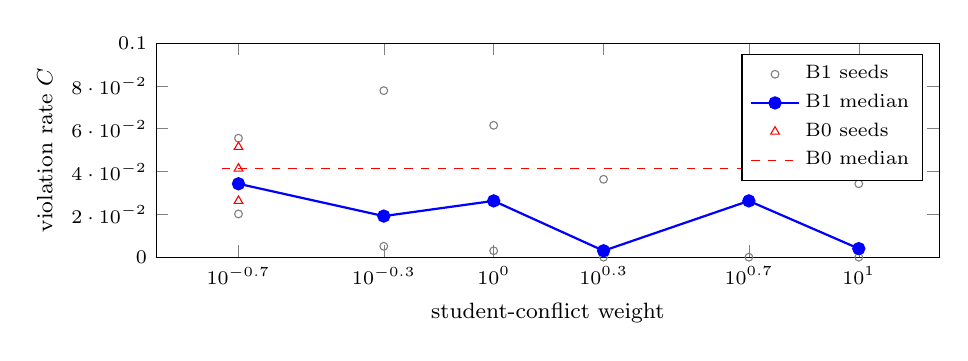
\begin{tikzpicture}
\begin{axis}[
    width=0.95\linewidth, height=4.3cm,
    xlabel={\footnotesize student-conflict weight},
    ylabel={\footnotesize violation rate $C$},
    xtick={0.2,0.5,1,2,5,10},
    xmode=log, log basis x=10,
    ymin=0, ymax=0.10,
    tick label style={font=\scriptsize},
    label style={font=\footnotesize},
    legend style={font=\scriptsize, at={(0.98,0.95)}, anchor=north east},
    legend cell align=left
]
\addplot[only marks, mark=o, color=gray, mark size=1.4pt] coordinates {
 (0.2,0.0343) (0.2,0.0556) (0.2,0.0202)
 (0.5,0.0192) (0.5,0.0051) (0.5,0.0778)
 (1,0.0616) (1,0.0030) (1,0.0263)
 (2,0.0364) (2,0.0030) (2,0.0000)
 (5,0.0263) (5,0.0000) (5,0.0444)
 (10,0.0343) (10,0.0000) (10,0.0040)
};
\addlegendentry{B1 seeds}
\addplot[mark=*, thick, color=blue] coordinates {
 (0.2,0.0343) (0.5,0.0192) (1,0.0263) (2,0.0030) (5,0.0263) (10,0.0040)
};
\addlegendentry{B1 median}
\addplot[only marks, mark=triangle, color=red, mark size=1.8pt] coordinates {
 (0.2,0.0414) (0.2,0.0263) (0.2,0.0515)
};
\addlegendentry{B0 seeds}
\addplot[dashed, color=red, domain=0.18:11] {0.0414};
\addlegendentry{B0 median}
\end{axis}
\end{tikzpicture}
\caption{Student violation rate against the student-conflict weight, on a fixed instance with a 900-second budget and three seeds per weight. Open circles are the B1 seeds in the per-seed metric files. Triangles are the B0 seeds at weight 0.2, namely 0.0414, 0.0263 and 0.0515; their median is the dashed line. The median of every weight at or above 0.5 lies below that line. The median drawn at weight 5 is the value recomputed from those files, 0.0263, rather than the archived summary value of 0. Two B1 seeds remain above 0.06.}
\label{fig:sweep}
\end{figure}

Two observations follow. First, the solver starts from $C=0.5313$ and the median of every weight falls below $0.06$ within the time budget while keeping all 262 classes assigned, so the overwhelming majority of the reduction comes from the search itself rather than from the weight. Two individual B1 seeds do not: 0.0778 at weight 0.5 and 0.0616 at weight 1. Second, the weight matters at the margin regardless of which reading of the weight-5 row is taken: measured against the B0 median of $0.0414$, the best setting reduces the residual rate by either $100\%$ (weight 5, as archived) or $92.7\%$ (weight 2, recomputed), and both readings clear by a wide margin the $25\%$ relative-improvement threshold that had been fixed in advance for the reinforcement-learning experiment of Section~\ref{sec:rl}.

\subsection{The final solution under pinned enrolments}
\label{sec:final}
With \emph{Enrolled Student Course Demands} selected and student switching disabled, the solver can no longer improve the conflict count by moving students, and the measurement becomes a property of the timetable alone. The exported solution was scored against the current dataset; Table~\ref{tab:final} gives the full evaluation and Fig.~\ref{fig:hardchecks} the hard-check pass rates.

\begin{table}[t]
\centering
\caption{Full evaluation of the final solution: 291 classes, 1{,}130 students, 42 rooms, 115 staff.}
\label{tab:final}
\footnotesize
\begin{tabular}{@{}lrr@{}}
\toprule
Metric & Value & Rate \\
\midrule
Coverage & 290 / 291 assigned & 99.66\% \\
Hard feasibility score & 98.85 / 100 & --- \\
Hard checks / failures & 4{,}341 / 105 & --- \\
Time-pattern fidelity & 290 / 290 & 100\% \\
Date pattern & 290 / 290 & 100\% \\
Room capacity & 290 / 290 & 100\% \\
Lunch / weekend compliance & 290 / 290 & 100\% \\
Instructor double-booking & 0 conflicts & 100\% \\
Room double-booking & 0 conflicts & 100\% \\
Student conflicts & 40 / 1{,}130 students (40 pairs) & 96.46\% \\
Student lunch breaks & 63 violations & 94.42\% \\
Instructor lunch breaks & 1 violation & 97.92\% \\
Preference score$^{\ddagger}$ & 6.29 / 100 & --- \\
\quad room preference & 35 / 278 & 12.59\% \\
\quad instructor identity$^{\dagger}$ & 0 / 289 & 0\% \\
\bottomrule
\end{tabular}
\\[2pt]
\raggedright\footnotesize $^{\ddagger}$Equal-weight mean of the two rates listed beneath it: $(12.59+0)/2=6.29$. $^{\dagger}$Name-format artefact, not a scheduling failure; see Section~\ref{sec:discussion}.
\end{table}

\begin{figure}[t]
\centering
\resizebox{\linewidth}{!}{%
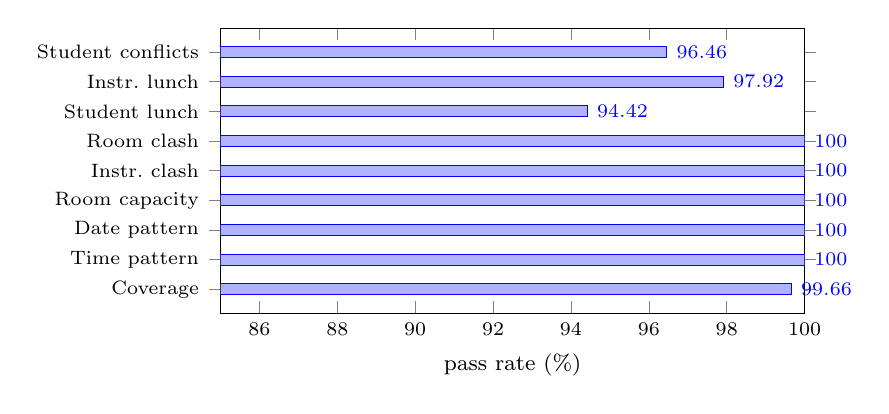
\begin{tikzpicture}
\begin{axis}[
    width=9cm, height=5.2cm,
    xbar, bar width=4pt,
    xmin=85, xmax=100,
    y dir=reverse,
    ytick=data,
    symbolic y coords={StudentConflicts, InstrLunch, StudentLunch, RoomClash, InstrClash, RoomCapacity, DatePattern, TimePattern, Coverage},
    yticklabels={Student conflicts, Instr.\ lunch, Student lunch, Room clash, Instr.\ clash, Room capacity, Date pattern, Time pattern, Coverage},
    tick label style={font=\scriptsize},
    nodes near coords, nodes near coords align={horizontal},
    every node near coord/.append style={font=\scriptsize},
    xlabel={\footnotesize pass rate (\%)}, label style={font=\footnotesize}
]
\addplot coordinates {
 (96.46,StudentConflicts)
 (97.92,InstrLunch)
 (94.42,StudentLunch)
 (100,RoomClash)
 (100,InstrClash)
 (100,RoomCapacity)
 (100,DatePattern)
 (100,TimePattern)
 (99.66,Coverage)
};
\end{axis}
\end{tikzpicture}}
\caption{Hard-check pass rates of the final solution. The horizontal axis starts at 85\% to make the three non-perfect checks legible.}
\label{fig:hardchecks}
\end{figure}

The timetable is hard-feasible in every respect the institution treats as non-negotiable: no room or instructor is double-booked, every class respects its meeting pattern and room capacity, and 290 of 291 classes are placed. The remaining 40 student conflicts are concentrated rather than diffuse: all 40 are first-year students, and all arise from the same pair of course types---a first-year programming laboratory overlapping the first-year reserved lecture block---across four specific laboratory/lecture combinations. Because the conflicts sit in four placements rather than being spread across the cohort, they are addressable either by re-timing those four laboratories or by adding explicit different-time distribution constraints between the laboratory subpart and the reserved block; neither remedy has yet been implemented or measured. The room-preference rate of 12.59\% is the clearest remaining optimisation target and reflects that room preferences were generated permissively from the source associations, leaving the solver free to trade them away cheaply.

\section{Reinforcement-Learning Control Experiment}
\label{sec:rl}

The weight sweep of Section~\ref{sec:weight-sweep} tunes a single scalar. A more ambitious question is whether the solver's choice of search move can itself be learned: at each step, CPSolver's neighbourhood selector picks a kind of move---change a time, change a room, swap two classes, request a suggestion---according to fixed probabilities, and the hypothesis tested here was that a policy conditioned on the state of the search could choose better than those fixed probabilities, reaching a lower student-conflict rate within the same time budget. A success criterion was fixed in advance: a learned policy would be judged to have succeeded only if it reduced the student violation rate by at least $25\%$ relative to a tuned baseline, at equal wall-clock budget, on a held-out instance. Fixing this threshold before running the experiment is what makes the result below meaningful rather than a post-hoc rationalisation.

The search is modelled as a Markov decision process~\cite{sutton2018rl} in which an agent observes a state, chooses an action, and receives a reward that depends on the resulting state. The agent is consulted once every fifty solver iterations rather than at every iteration, which keeps the inference cost negligible against the cost of the search itself. The state is a 48-dimensional real vector grouped into conflict features (violation rate, pair rate, intensity, and concentration), a ten-bin histogram of conflict load across the day, search-progress features such as the acceptance rate and recent improvement slope, solution features (assigned ratio and the normalised room, time, and distribution criteria), room and instructor utilisation, and a record of the previous operator chosen. The reward is a potential-based shaping term over the incumbent solution that combines the student violation rate, the unassigned fraction, the count of hard violations, and the normalised soft objective into a single scalar, with the step reward defined as the change in that potential between successive decision points less a small constant to discourage stalling; potential-based shaping~\cite{ng1999shaping} was chosen specifically so that the reward signal is dense without altering the ordering of final solutions it would otherwise compare. The trained policy uses proximal policy optimisation~\cite{schulman2017ppo} with invalid actions masked out~\cite{schulte2017maskable}. An online alternative, not a neural network, is LinUCB~\cite{li2010linucb}, a linear contextual bandit in the upper-confidence-bound family~\cite{auer2002ucb}.

The layer was implemented as CPSolver's own move-selection extension point, which matters for safety: nothing in the layer writes a placement directly. Every candidate move is produced by a stock CPSolver generator and is then accepted or rejected by CPSolver's own acceptance criterion exactly as in an ordinary solve, so a learned policy can make the search slower or less effective, but it cannot make the timetable illegal. The implementation comprises 25 Java classes and 11 Python modules: a 48-dimensional state encoder, eight neighbourhood operators (six stock CPSolver generators and two written for this project to bias sampling toward classes and students already in conflict), a potential-based reward shaping term over the incumbent solution, a gRPC training environment, and an ONNX inference path that runs the frozen policy inside the solver's own Java virtual machine with a timeout and a fallback to the stock selector.

The outcome is a negative result, and the project treats it as such rather than as a setback to be explained away. Arm B1 exists precisely to ask whether the stock objective was simply under-weighted, and Section~\ref{sec:weight-sweep} shows that it was: raising the student-conflict weight on a fixed instance took the median violation rate from $0.0414$ to $0.0030$ or below, a reduction well past the $25\%$ bar the learned policy had been set to clear. The only bake-off conducted on a real institutional instance compared the baseline arms alone, and that instance was already conflict-free when loaded, so it could not have separated a learned policy from a fixed one even had both been run. Measurement on a small synthetic instance (120 classes, 600 students, 6 rooms) confirmed that the training pipeline runs end to end---roughly 100 macro-steps per second per worker, an ONNX forward pass of about 0.08\,ms, and a PyTorch--ONNX numerical deviation of $2\times10^{-6}$---but every arm tied at the same violation rate on that instance and a behaviour-cloned policy was markedly worse, having collapsed onto a single operator; the project's own notes describe this as a pipeline check rather than evidence of anything about search quality, and this paper treats it the same way. The learned policy was never run on an institutional instance at all.

Two further points limit how this null result should be read. First, the synthetic-instance check above is a pipeline check and not a search-quality result precisely because the comparison that matters---learned policy against tuned baseline, on an institutional instance, at a held-out term---was never run; everything that can be said about search quality on real data rests on Section~\ref{sec:weight-sweep} alone. Second, the layer's own design invariant, that every move it proposes must still be generated and accepted by stock CPSolver machinery, means the worst a mis-trained policy can do is waste search budget, not produce an illegal or materially worse timetable, which is why it was safe to leave the layer fully instrumented and partially evaluated rather than withdrawing it once the control experiment answered the research question.

No claim is therefore made that the learned policy outperforms the tuned baseline. On this instance and at this budget, the residual conflicts after search came from how the objective was priced, not from how the search explored, and a correctly configured stock solver already suffices. The conflict oracle, state encoder, and headless runner built for this layer remain useful independent of that conclusion, since cross-validating the oracle against the Python evaluator (Section~\ref{sec:evaluator}) is what made the controlled weight comparison in Section~\ref{sec:weight-sweep} trustworthy in the first place, and the infrastructure is ready should a larger, harder instance turn out not to yield to weight tuning alone.

\section{Discussion}
\label{sec:discussion}

The results above hold under conditions that should be stated plainly rather than left implicit.

\emph{The student body is simulated.} No MIS data was available, so all 1{,}130 students are generated from confirmed headcounts and deterministic enrolment rules rather than real course choices. Elective demand in particular is modelled as an even split across options, whereas real demand is typically skewed; a skewed distribution would place more students in the larger sections and could change which overlaps matter. A small number of known defects follow from this simulation and from the section-filling order used to build it: two hundred first-year students could not be placed in one programming-laboratory offering because the declared section limits do not cover the cohort, two postgraduate students overflow one laboratory, and three final-year laboratory batches end up mixed across lecture divisions because the preferred batches of one division filled first---creating joint enrolments the institution does not actually intend, and with them, conflict opportunities that a correct section structure would not have produced.

\emph{The residual conflicts are diagnosed but not fixed.} The 40 first-year conflicts reported in Section~\ref{sec:final} are localised to four laboratory placements against the reserved lecture block, and two remedies were identified---re-timing those laboratories, or adding explicit different-time distribution constraints---but neither has been implemented or measured, so the number in Table~\ref{tab:final} should be read as a diagnosed, addressable residue rather than a quality ceiling.

\emph{Soft-constraint quality is poor and the preference aggregate is partly uninformative.} The room-preference hit rate of 12.59\% is a genuine optimisation gap: no tuning of the room-preference weight relative to the student-conflict weight was attempted, in contrast with the controlled sweep performed for the latter. The instructor-identity check, by contrast, scores 0\% for a reason that has nothing to do with scheduling quality: UniTime exports instructor names in last-initial form, while the comparison data uses full names, so every class fails a check that compares two different renderings of the same identity. The underlying assignment is correct, and the aggregate preference score of 6.29 out of 100 should not be quoted on its own because this one broken, equally-weighted check drags it down disproportionately.

\emph{Scope is one department and one term.} Everything reported here concerns Computer Engineering for a single academic session; a university-wide instance would be several times larger and would introduce inter-departmental room contention this dataset does not exercise.

\emph{The evaluator's own aggregate is a double-edged design choice.} Weighting every hard check equally makes the headline feasibility score easy to interpret, but it also means a single structurally broken check, such as the instructor-identity comparison above, can swing the number without any change to the underlying schedule. This is not a flaw unique to this project: any equal-weight aggregate over heterogeneous checks will behave the same way, and the only general remedy is the one adopted here, which is to always publish the component rates beside the aggregate rather than the aggregate alone.

\emph{Generalisation beyond this instance is untested.} Every number in Sections~\ref{sec:results} and~\ref{sec:rl}, including the weight sweep and the reinforcement-learning control experiment, was measured on one department's data for one term. Nothing in the pipeline is specific to that department---the generators are parameterised by snapshot and academic term---but no second, independently sized instance was solved and scored end to end during this phase, so claims about how the residual conflict rate or the weight sensitivity would behave on a larger or structurally different instance remain extrapolations rather than measurements.

\emph{Software stack.} For completeness: the UniTime server itself runs on Java 21, while Java 17 is only the compile target declared for this project's own reinforcement-learning module and headless tooling, which run unchanged on Java 21 since bytecode compiled for release 17 is backward-compatible; no component requires a version downgrade.

Read together, these caveats point in one direction: the measurement machinery---the independent evaluator, its cross-validated conflict rule, and the pinned-enrolment protocol---is the more durable contribution of this phase, because it is what turned four previously unfalsifiable "zero-conflict" claims into one honest, small, and diagnosable number.

\section{Conclusion}
\label{sec:conclusion}

A preceding feasibility phase established that UniTime's constraint model is expressive enough to represent every scheduling rule in force at this department; that was a statement about the platform. The phase reported here turned it into a working system and, in doing so, produced a measured timetable rather than a feasibility argument. A reproducible pipeline reads a snapshot of the institution's existing scheduling database and emits the sixteen ordered documents UniTime requires, covering one session, 42 rooms across six buildings, 115 instructors, 56 offerings comprising 291 classes, and a simulated body of 1{,}130 students with 9{,}148 section enrolments, behind validators that refuse to produce an archive from inconsistent data. The institution's own rules, including the minor-degree and open-elective block times and the dynamic lunch window, are generated as data rather than re-entered after each import. An independent evaluator scores any exported timetable against the same input files, using a conflict definition cross-validated against a separate implementation to exact numerical agreement.

The substantive result concerns measurement as much as optimisation. Several configurations reported zero student conflicts, and each was traced to an artefact: students silently re-sectioned between laboratory batches, an instance that was already conflict-free, or a solver that had loaded no students at all. Pinning the enrolments removed the solver's ability to improve the reported number by moving students instead of classes, and the count rose from an apparent zero to a real 40. That rise was the objective, not a regression. The final solution places 290 of 291 classes with no instructor or room double-booking, a hard feasibility score of 98.85 out of 100, and 40 of 1{,}130 students conflicted, all first-year students in four laboratory placements against a single reserved lecture block---a scheduling problem with a known shape rather than a quality ceiling.

A reinforcement-learning layer that selects among CPSolver's neighbourhood operators was implemented in full and designed so that it can never produce an illegal timetable, since every move it proposes is generated and accepted by stock CPSolver machinery. Its pre-registered control experiment answered the project's own research question in the negative: raising the student-conflict weight on a fixed instance already reduces the median violation rate by well over the $25\%$ threshold the learned policy had been set to beat, so no claim is made that learning outperforms a correctly tuned baseline here. The useful conclusion is narrower and more durable than either a positive or a negative headline result alone: for an instance of this size, the residual student conflicts were a consequence of how the objective was priced, not of how the search explored, and a correctly configured stock solver is sufficient. What remains before this system could be adopted operationally is a return path from a solved timetable back into the institution's live scheduling database, a student data source drawn from the MIS portal rather than simulated, and an extension of scope beyond one department and one term---three well-defined tasks rather than open questions. None of the three is blocked on anything reported here: the pipeline is already parameterised by snapshot and term rather than hard-coded to this department's data, the evaluator already treats the solver as a black box and would score a university-wide export the same way it scores this one, and the only reason the first-year conflicts remain unresolved is that doing so was out of scope for this phase rather than out of reach of the tooling built for it. The more general lesson, independent of this particular department or dataset, is that a scheduler's self-reported quality metric should never be trusted without an evaluator built to the same standard of independence used here---one that is handed a timetable and a set of enrolments and nothing else, and that therefore cannot be fooled by whatever the solver did internally to arrive at the number it would rather report.

\section*{Acknowledgment}
The authors thank their project guide, Abhijit~A.~M., for supervision throughout this phase, and the department for providing the Taasika database snapshots used throughout this study.

\bibliographystyle{IEEEtran}
\bibliography{references(1)}

\end{document}
